\section{Hyper parameter tuning} \label{ch:hyper_parameter_tuning}

Unfortunately there is no obvious optimal model for every problem.
A model maps the input to the output, but to reliably determine which information in the data should be discarded (and thus not contribute to generalization) and which should be emphasized, appropriate assumptions must be made.

In 1996 David Wolpert pointed out that there is no reason to prefer one model over another if no assumptions are made about the data set.
This line of argument is now known as the \textit{No Free Lunch Theorem} \cite{Wolpert1996}.
Some of these assumptions are made in advance (for example, the use of feed-forward neural networks), but others are subject to optimization.

Hyperparameter optimization is an optimization problem in which the loss (or other metrics such as the accuracy) of the model for the given training data is to be minimized.
The hyperparameters used in the first model, which could be the subject of optimization, are among others:

\begin{enumerate}
    \item Training data:
    \begin{tasks}(2)
        \task Number of training examples
        \task Image size
        \task Batch size
        \task Feature reduction
    \end{tasks}
    \item Model:
    \begin{tasks}(2)
        \task Number of layers
        \task Layer type
        \task Layer size
        \task Loss function
    \end{tasks}
    \item Optimizer:
    \begin{tasks}(2)
        \task Type of optimizer
        \task Learning rate
        \task Momentum
        \task Nesterov
    \end{tasks}
    \item Training:
    \begin{tasks}(2)
        \task Steps per epoch
        \task Number of epochs
    \end{tasks}
\end{enumerate}

Some hyperparameters need to be tested and are not obvious, but others can be improved without obvious negative side effects, so they are discussed here first. Then, algorithms for testing different models with different hyperparameters to improve the model will be studied.

\subsection{Data augmentation}\label{ch:data_augmentation}

% TODO Add citation to Chollet p.138
% TODO Add dropout layer Chollet p.140
The first thing that can be improved is the size of the dataset we use to train the model.
In previous tests, the models saw each image about 20 times during training (batches of size 20, 20 steps per epoch, and 20 epochs divided by 400 training samples), which is most likely the cause of the overfitting that occurs.
So increasing the size of the training batch seems to be a reasonable approach.

The augmentation of the data works in this case by changing some properties of the image that are useful for the purpose.
In the case of symbol recognition, the symbol can be rotated or mirrored so adding training examples without adding much redundancy to the dataset and in this very case not invalidating the data.

The data extension is done by adapting the \code{create\_generator} function previously used:

\begin{lstlisting}
from tensorflow.keras.preprocessing.image import ImageDataGenerator

def create_generator(data_dir, batch_size, datagen):
    full_path = join(processed, data_dir)
    return datagen.flow_from_directory(
        full_path,
        target_size=(32, 32),
        batch_size=batch_size,
        class_mode='binary')

train_datagen = ImageDataGenerator(
        rescale = 1./255,
        rotation_range=360,
        horizontal_flip=True,
        vertical_flip=True)

test_datagen = ImageDataGenerator(rescale = 1./255)

train_generator = create_generator('train', 20, train_datagen)
test_generator = create_generator('test', 10, test_datagen)
\end{lstlisting}

Instead of \code{datagen = ImageDataGenerator(rescale = 1./255)} this object is specified as parameter, because the training set makes random changes to the loaded data.
Namely a random rotation and the possibility to be mirrored horizontally and vertically.
Please note that no changes are applied to the test data.

Applying these changes results in a loss of 0.61 and a 78.75\% accuracy of the training data.
The loss and accuracy of the test set is 0.63 and 78\% respectively.

\begin{figure}
    \centering
    \begin{subfigure}[b]{0.4\textwidth}
        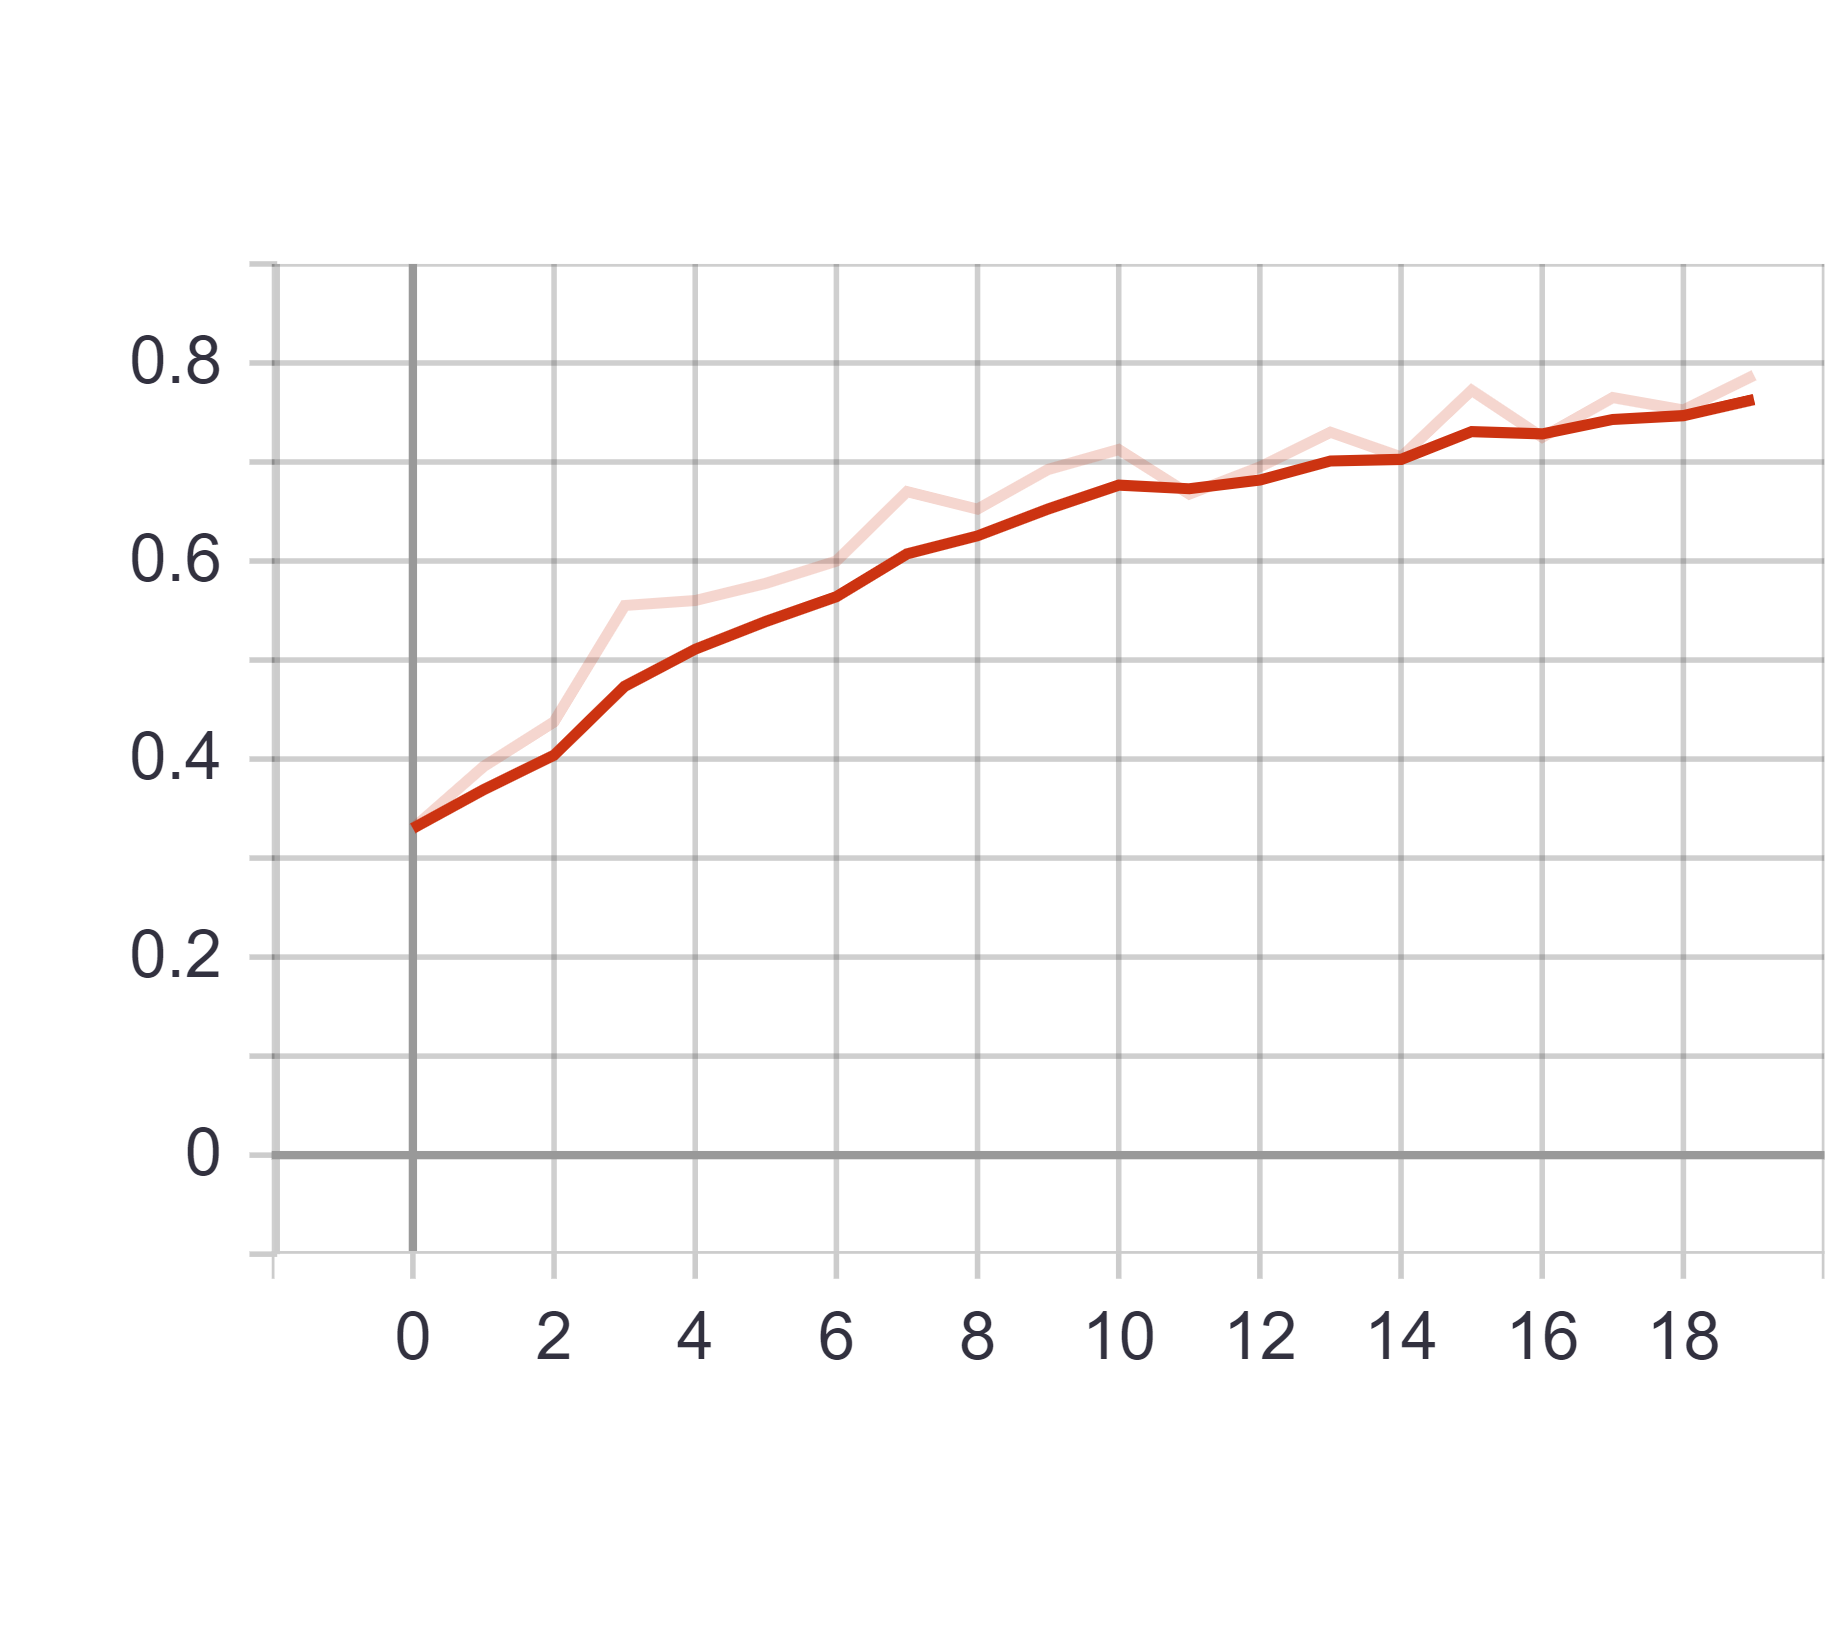
\includegraphics[width=\textwidth]{images/first_model_data_augmentation_acc.png}
        \caption{Accuracy}
        \label{fig:first_model_data_augmentation_acc}
    \end{subfigure}
    \begin{subfigure}[b]{0.4\textwidth}
        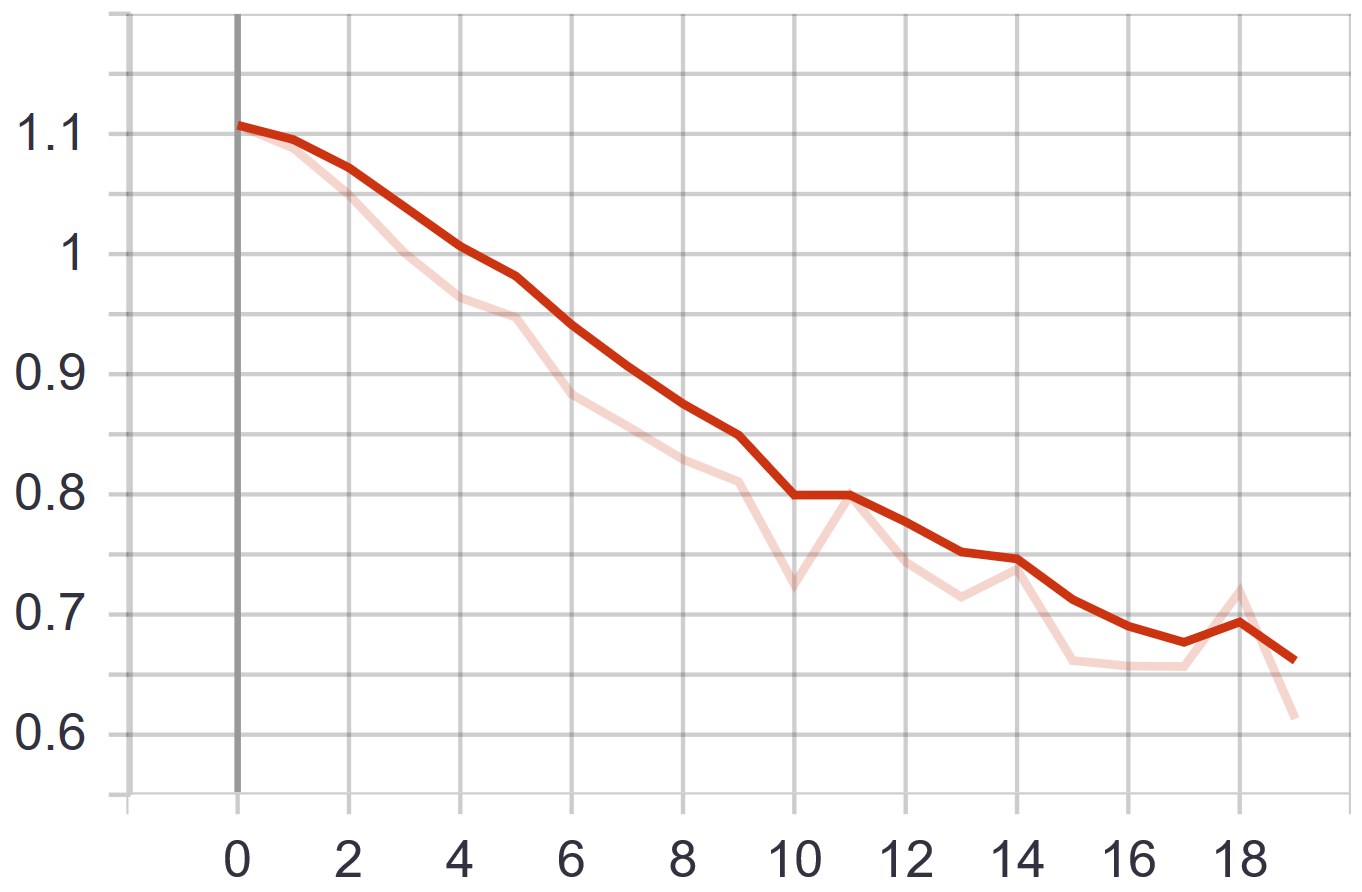
\includegraphics[width=\textwidth]{images/first_model_data_augmentation_loss.png}
        \caption{Loss}
        \label{fig:first_model_data_augmentation_loss}
    \end{subfigure}
    \caption{Compared to figure~\ref{fig:first_model_graphs}, accuracy and loss increases more slowly. Further epochs may improve the results, as the model does not seem to have fully converged after 20 epochs.}
    \label{fig:first_model_data_augmentation_graphs}
\end{figure}

It is obvious that the accuracy of the training data actually decreases here.
This is not surprising, as the model is no longer given data twice, i.e. there is no memorization, but as the test accuracy has not changed, the desired effect seems to have occurred.
The model accuracy of the training set also seems to increase at a lower rate, so that more epochs or larger batches could already improve the performance.

Please note that the training set has practically grown by a factor of 1440 (360 degrees + rotations in two axes), which makes it possible to feed considerably more data into the model during training without having to expect too much overfitting.

The goal of reducing overfitting seems to be solved in this regard; the difference between training and test accuracy is negligible\footnote{link to the respective notebook: \url{https://aka.klawr.de/srp\#7}}.

\subsection{Feature reduction}

Another thing that can improve the performance of the model is to reduce the size of the input.
The phenomenon known as \textit{curses of dimensionality} describes the possibilities of different configurations that are possible with an increasing number of variables, and comes from Richard Bellman, who first refers to problems in dynamic programming \cite[p.ix]{Bellman1957}.

The data is already greatly reduced by loading the data as images with a width and height of 32 pixels, although the data is raw as 512 by 512 images. This reduction has been done manually beforehand to keep the data relatively small, but the symbols are still clearly distinguishable.

Although the raw data contains only grayscale colors, the images are loaded with three color channels (hence the input size \code{[32, 32, 3]}).
So one way to reduce the input size is to project the data onto a color dimension, as suggested by Géron \cite[p.215]{Geron2019}.
The call of the \code{flow\_from\_directory} is thus supplemented by a further parameter \code{color\_mode='grayscale'} with the 3-dimensional \code{color\_mode='rgb'} (which is set as default) to one dimension.
Practically nothing should change, except the input size, which is adjusted to \code{[32, 32, 1]}.

The resulting model accordingly looks as follows:

\begin{lstlisting}
Model: "sequential"
_________________________________________________________________
Layer (type)                 Output Shape              Param #   
=================================================================
flatten (Flatten)            (None, 1024)              0         
_________________________________________________________________
dense (Dense)                (None, 32)                32800     
_________________________________________________________________
dense_1 (Dense)              (None, 32)                1056      
_________________________________________________________________
dense_2 (Dense)              (None, 3)                 99        
=================================================================
Total params: 33,955
Trainable params: 33,955
Non-trainable params: 0
_________________________________________________________________
\end{lstlisting}

The number of trainable parameters is almost divided by a factor of three, reducing the size of the model from 807kb (from the previous models with 99491 parameters) to 295kb.
Nevertheless, no accuracy is lost. \footnote{Link to the respective notebook: \url{https://aka.klawr.de/srp\#8}}.

\subsection{Optimizers}

So far only the optimizer of stochastic gradient descent has been considered.
The stochastic gradient descent has several parameters that can be optimized, e.g. the learning rate, the momentum and whether Nesterov is used or not, as discussed in chapter~\ref{ch:optimizer}.

Several attempts have already been made to automate the search for these hyperparameters.
In this project some alternative optimizers are investigated, but not explained in too much detail.
Please refer to the given citations for further insights.

With stochastic gradient descent, the learning rate is the same for all parameters of every layer in the model.
An adjustment for each parameter or even for individual dimensions of the layers can be helpful, but to do this manually would require a disproportionate effort.

\name{AdaGrad} \cite{Duchi2010} changes the learning rate for each parameter.
This is done by adjusting the learning rate (starting with a uniform value) for each individual parameter using the size of the gradient for the respective parameter.
While this approach works well for some problems, it does not make sense for some problems.
Nevertheless, it serves as a baseline for many other optimizers developed after it, three of which have been tested in the tuning algorithm used in this project.

\name{AdaDelta} \cite{Zeiler2012} is a modified algorithm based on \name{AdaGrad} that tries to solve AdaGrad's idea of constantly reducing the learning rate by dividing the learning rate again by an exponentially decreasing average (decay) of the gradients.
This leads to a much more stable optimizer that promises to work well in practice.

\name{RMSProp} \cite{Hinton2012} works similar to \name{AdaDelta} with a slightly different update rule.
It is considered to be "generally a good enough choice, whatever your problem". \cite [p.77]{Chollet2017}.

Adam \cite{Kingma2014}\cite{Reddi2018} is the last optimizer included in this project, which is another method to apply an adaptive learning rate for each parameter.
Adam integrates the aforementioned idea of momentum into an algorithm similar to that of \name{RMSProp}.

There are other optimizers worth mentioning (namely AdaMax or Nadam), which may be the subject of further investigation.

It is remarkable that the adaptive methods explained here may not work with every model, so that it is always worth trying the basic gradient descent with nesterov\cite [p.358]{Geron2019}.

\subsection{Convolutional layers}

Convolutional layers are widely used for image recognition and it is therefore useful to integrate them into this model.
They were introduced by Yann LeCun in 1998 in a work \cite{Lecun1998} to recognize handwritten numbers.

In this project only two-dimensional convolutional layers are used, because the input is two-dimensional (after the images have been transferred in grayscale).
The difference between the convolutional layers and the previously described "Dense Layers" is that the trained parameters do not represent the connections of all nodes of the previous layer to a next one, but a kernel that slides over the input layer and acts as a filter that builds up the output layer.
This also means that the input layer does not need to be flattened before it is fed into the model.

When training a convolutional layer, the trained parameters are the filters that have a given shape.
A two-dimensional convolutional layer with eight filters, an input depth of one and a kernel size of four times four (and one for the bias) has 136 (8 x (1 x 4 x 4 + 1)) parameters, which is significantly less than with previous approaches and does not depend on the size of the input layer, so that it is possible to recognize patterns in images of any size without having to enlarge the model itself.

The corresponding equation for a single activation is therefore given by \cite [p. 453]{Geron2019}:
\begin{equation}
z_{i,j,k} = b_k + \sum_{u=1}^{h} \sum_{v=1}^{w} \sum_{k'=1}^{n'} x_{i', j', k'} \times w_{u, v, k', k} 
\end{equation}

Where $z$ is the activation value, the indices $i$ and $j$ represent the position of the node in the output layer and $k$ the index of the filter.
The sum of all input nodes is the sum of the nodes in the respective directions given by iteration over three axes using the height ($h$), width ($w$) and filter size ($n'$) of the previous layer.
For each of these combinations, the respective connection weight $w_{u, v, k', k}$ is multiplied by the input $x_{i', j', k'}$ at the respective position in the previous layer, where $i' = i \times s_h + u$ and $j' = j \times s_w$ respectively, and $s_h$ and $s_w$ are the steps taken at each step in each direction.
The steps reduce the size of the following layer.
Additionally, each filter has its own bias $b_k$, which is added to the activation function.

\begin{figure}
    \centering
    \caption{  The bottom layer is the input, which is represented by a two-dimensional layer of size five by five (filter size is one), padded with a padding of one (drawn in gray) to ensure that the size remains the same when using a kernel of size three by three (highlighted by the red, green and blue rectangles). The stride used is one, i.e. the receptive field propagates one input node at each step. Here the process starts at the red rectangle, blue is the second step and green the last (25 steps in total). }
    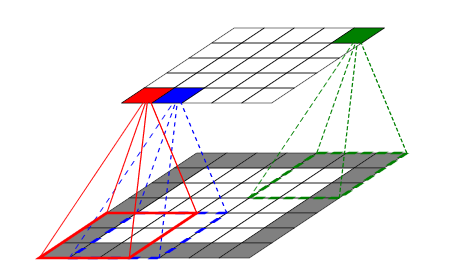
\includegraphics[width=0.6\textwidth]{images/conv_layer.png}
    \label{fig:conv_layer}
\end{figure}

In order for the output to be the same size as the input, numbers must be added to the input, since a kernel that is greater than one in any direction cannot cross an edge for the input (and the step must be 1 by 1).
So padding is used to solve this problem by (typically) adding zeros around the input, resulting in a technique called zero padding.

By using convolutional layers instead of dense layers, the model size is further reduced (295kb to 232kb) and accuracy is increased by a few percent. Adding pooling reduces the size further to 149kb and further improves the accuracy\footnote{Link to the respective notebooks: \url{https://aka.klawr.de/srp\#9} and \url{https://aka.klawr.de/srp\#10}.
Pooling is a technique where a kernel (similar to the core of Convolutional Layers) scans over the input layer}.
In the linked notebook, a kernel was used in pairs, taking the maximum value of the kernel and passing only the maximum value, thus halving the output size in width and height\footnote{This is appropriately called \name{MaxPooling}.}.

\subsection{Tuning algorithms}

Taking into account all possibilities to optimize the model before training, some approaches have been developed to automatically optimize the hyperparameters.
One way of setting the hyperparameters is to test each one with different values, but freezing the values of all other hyperparameters.
This is then repeated for all hyperparameters.
This procedure ensures that the optimal set of hyperparameters is used, but can take an unacceptable amount of time, since the number of models created grows exponentially with the number of hyperparameters to be adjusted.
With two hyperparameters, this would mean checking each value on a two-dimensional grid, so the method is called "grid search"\footnote{If only one hyperparameter is adjusted, the method is called "linear search".}.

Another approach frequently used in practice is the random search.
The random search works on the principle of randomly assigning hyperparameters and thus testing different models without any advantage of a combination.
Of course, this (most likely) does not lead to an optimal result, but in practice this approach is often used because it usually gives an acceptable result by testing a wide range of possible configurations.
A notebook was created to show the implementation of \name{keras tuner} in this project at \url{https://aka.klawr.de/srp\#12}.

Some more sophisticated methods are based on the random search approach, in which the results of the random search are repeatedly examined and then the hyperparameters are adjusted in favor of those that promise to yield better models.
This approach is called zooming, because after each iteration you zoom into the most promising range of hyperparameters.

Other approaches try to completely automate this process.
Popular algorithms are based on Bayesian optimization, but these are not covered in this project and are therefore omitted.

The tuner used in this project is called \name{Hyperband} \cite{Li2018}, which is implemented in the library \name{keras-tuner}. \cite{Google2019a}.
Essentially, \name{Hyperband} trains models using random searches, but restricts training to a wide range of hyperparameters in a few epochs.
This is done by training the models for a few epochs and keeping only the most promising models for further iterations.
This method promises a much better use of resources and will most likely be able to present good hyperparameters.

The final model tuner is designed to accept a \code{Hyperparameter} object that is supplied to a function that returns the respective model:

% TODO python
\begin{lstlisting}
def create_model(hp):
    model = models.Sequential()
    model.add(layers.Conv2D(2**hp.Int('2**num_filter_0', 4, 6),
        (4,4) ,activation='relu', input_shape=(32, 32, 1)))

    for i in range(hp.Int('num_cnn_layers', 0, 3)):
        filter = 2**hp.Int('2**num_filter_' + str(i), 4, 7)
        model.add(
            layers.Conv2D(filter, (4,4), activation='relu',padding='same'))
        if hp.Boolean('pooling_' + str(i)):
            model.add(layers.MaxPooling2D(2, 2))

    model.add(layers.Flatten())
    for i in range(hp.Int('num_dense_layers', 1, 3)):
        nodes = 2**hp.Int('2**num_nodes_' + str(i), 4, 7)
        model.add(layers.Dense(nodes, activation='relu'))
    
    model.add(layers.Dense(3, 'softmax'))

    optimizers = {
        'adam': Adam(),
        'sgd': SGD(lr=hp.Choice(
            'learning_rate', [0.001, 0.003, 0.007, 0.01 0.03]),
            momentum=hp.Float('momentum', 0.6, 1, 0.1),
            nesterov=hp.Boolean('nesterov')),
        'rms': RMSprop(lr=hp.Choice(
            'learning_rate', [0.001, 0.003, 0.007,0.01, 0.03]))
    }

    model.compile(
        loss='sparse_categorical_crossentropy',
        optimizer=optimizers[hp.Choice('optimizer', list(optimizers.keys())],
        metrics=['acc'])

    return model
\end{lstlisting}

This function extends \ref{lst:first_model} by implementing hyperparameters using \code{hyperparameter} of \name{keras tuner}.
This will be implemented later using a custom class\footnote{The results are logged with \name{TensorBoard}, whose API is not yet supported by \name{keras tuner} itself. So the tuner is inherited from a custom class}:

\begin{lstlisting}
tuner = customTuner(
    create_model,
    hyperparameters=hp,
    objective='acc',
    max_trials=100,
    executions_per_trial=1,
    directory=log_dir,
    project_name=timestamp)
\end{lstlisting}

The training that was previously performed by the \code{fit} function is now performed by the \code{search} function of the tuner:

\begin{lstlisting}
tuner.search(
    train_dataset,
    validation_data=validation_dataset,
    epochs=30,
    steps_per_epoch=100,
    validation_steps=100,
    verbose=0,
    callbacks=callbacks)
\end{lstlisting}

Another note to take here is that the generators used in \ref{ch:data_augmentation} have been replaced by custom functions to augment data. The data is then preprocessed using protocol buffers(\name{protobufs})\footnote{The final notebook using these can be found at \url{https://aka.klawr.de/srp\#11}}.
By pre-processing the image data in advance, the loading time of the data is significantly reduced.
The code used for this can be viewed here: \url{https://aka.klawr.de/srp\#13}.

After checking the data, an accuracy of 96.7\% on the test data was achieved with a model size of 4.3mb.

\subsection{Increasing the training set}

After the model was adapted, another approach was tried to increase the accuracy.
The raw training data was more than tripled (to 1000 examples for each symbol in the training data) and then expanded with 32 repetitions, resulting in a data set of 96000 different images.

Using this data set, almost every model tested previously achieved an accuracy of over 99\%.
This situation presents the minimization of the model as the most important optimization goal.
The final model is manually reduced and tuned by reducing layers and hyper parameters.
The final model has a size of 207kb with an accuracy of 99.3\% and a loss of 0.04 on the training set, which is satisfactory.

The model is summarized as:

\begin{lstlisting}
model = models.Sequential()
model.add(layers.Conv2D(16, (4,4), activation='relu', padding='same',
    input_shape=(32, 32, 1)))
model.add(layers.MaxPooling2D(2,2))
model.add(layers.Conv2D(32, (4,4), activation='relu', padding='same'))
model.add(layers.MaxPooling2D(2,2))
model.add(layers.Flatten())
model.add(layers.Dense(3, 'softmax'))

optimizer = Adam()
model.compile(loss='sparse_categorical_crossentropy',
    optimizer=optimizer,metrics=['acc'])
\end{lstlisting}

The code for the model creation can be viewed at \url{https://aka.klawr.de/srp\#14}.
